
%(BEGIN_QUESTION)
% Copyright 2010, Tony R. Kuphaldt, released under the Creative Commons Attribution License (v 1.0)
% This means you may do almost anything with this work of mine, so long as you give me proper credit

Suppose a thermocouple (producing a DC voltage as it heats up) is connected to a data acquisition module to record the temperature of a process:

$$\includegraphics[width=15.5cm]{i04564x01.eps}$$

The signal recorded by the DAQ unit is ``noisy,'' and you suspect 60 Hz AC interference may be coupling to the thermocouple cable from some external source.  Explain how you would use basic electronic test equipment (i.e. nothing more complex or specialized than what you would find in our first-year electronics lab) to confirm this was the problem, and also show on the diagram where you would connect this test equipment to perform the confirmation.

\underbar{file i04564}
%(END_QUESTION)





%(BEGIN_ANSWER)

I recommend half credit for identifying a suitable piece of test equipment (AC voltmeter or oscilloscope) and half credit for showing how to connect it (in parallel with the DAQ's thermocouple input terminals).

\vskip 10pt

Another possible solution (requiring {\it no} test equipment!) is to temporarily disconnect the shield conductor from ground and check to see if the noisy signal gets significantly noisier (as indicated by the DAQ).  If so, the problem is definitely induced noise from electric fields.

%(END_ANSWER)





%(BEGIN_NOTES)

{\bf This question is intended for exams only and not worksheets!}.

%(END_NOTES)

